\chapter{IMPLEMENTATION LEVEL UML} \label{ch:procedure}

\section{Implementation Level UML Class Diagram: Multi-Tenant E-Commerce System}

The Implementation Level UML Class Diagram for the Multi-Tenant E-Commerce System provides a detailed, code-oriented blueprint that translates the system's logical design into precise specifications for actual software implementation. This diagram serves as the definitive technical reference for developers during the coding phase.

\subsection*{Key Characteristics}

\begin{itemize}
    \item \textbf{Complete Class Specifications:} Each class includes fully defined attributes with exact data types (e.g., \texttt{String}, \texttt{Integer}, \texttt{Float}, \texttt{Boolean}, \texttt{DateTime}, \texttt{Decimal}), visibility indicators (\texttt{+} public, \texttt{-} private, \texttt{\#} protected), and method signatures with parameters and return types.
    
    \item \textbf{Multi-Tenant Architecture:} The diagram explicitly models the core requirement of data isolation through the central \texttt{Tenant} class, which associates with all tenant-specific entities. Each vendor's data (products, orders, customers) maintains a direct reference to its parent \texttt{Tenant}, ensuring strict segregation at the object level.
    
    \item \textbf{Database-Per-Tenant Pattern:} The \texttt{Tenant} class is associated with a\\ \texttt{DatabaseInstance} class, representing the physical or logical database allocated to each vendor. This enables the system to route queries to the appropriate database based on the tenant context.
    
    \item \textbf{Precise Relationships:} All associations between classes include multiplicity indicators (1, 0..*, 1..*, 0..1) that define cardinality constraints. Key relationships include:
    \begin{itemize}
        \item One-to-many: \texttt{Tenant} (1) $\rightarrow$ \texttt{Product} (0..*)
        \item Composition: \texttt{Order} (1) $\rightarrow$ \texttt{OrderItem} (1..*)
        \item Many-to-many: Resolved through association classes like \texttt{DiscountProduct}
    \end{itemize}
    
    \item \textbf{Modular Integration:} The diagram integrates classes from all five functional modules:
    \begin{itemize}
        \item \textbf{Vendor Management:} Tenant, Vendor, Customer, Order, Cart, Subscription
        \item \textbf{Product \& Inventory:} Product, Category, Inventory, StockMovement
        \item \textbf{Offers \& Customization:} Discount, Offer, Theme, StoreCustomization
        \item \textbf{Payment \& Delivery:} Payment, TransactionLog, Delivery, Shipment, CourierService
        \item \textbf{Communication \& Feedback:} Notification, Review, Rating, Campaign
    \end{itemize}
\end{itemize}

\subsection*{Purpose and Benefits}

\begin{itemize}
    \item \textbf{Code Generation:} Provides direct mapping to object-oriented programming languages (PHP/Laravel classes), enabling straightforward implementation.
    \item \textbf{Database Schema Design:} Serves as the foundation for creating relational database tables, with classes mapping to tables and attributes to columns.
    \item \textbf{API Contract Definition:} Method signatures define the operations available through the system's API endpoints.
    \item \textbf{Team Coordination:} Ensures all five team members develop consistent, interoperable classes that integrate seamlessly.
    \item \textbf{Validation and Testing:} Provides the basis for unit test case development and system validation.
\end{itemize}


\section{Multi-Tenant E-Commerce System UML Class Diagram (Implementation Level)}
\begin{figure}[H]
    \centering
    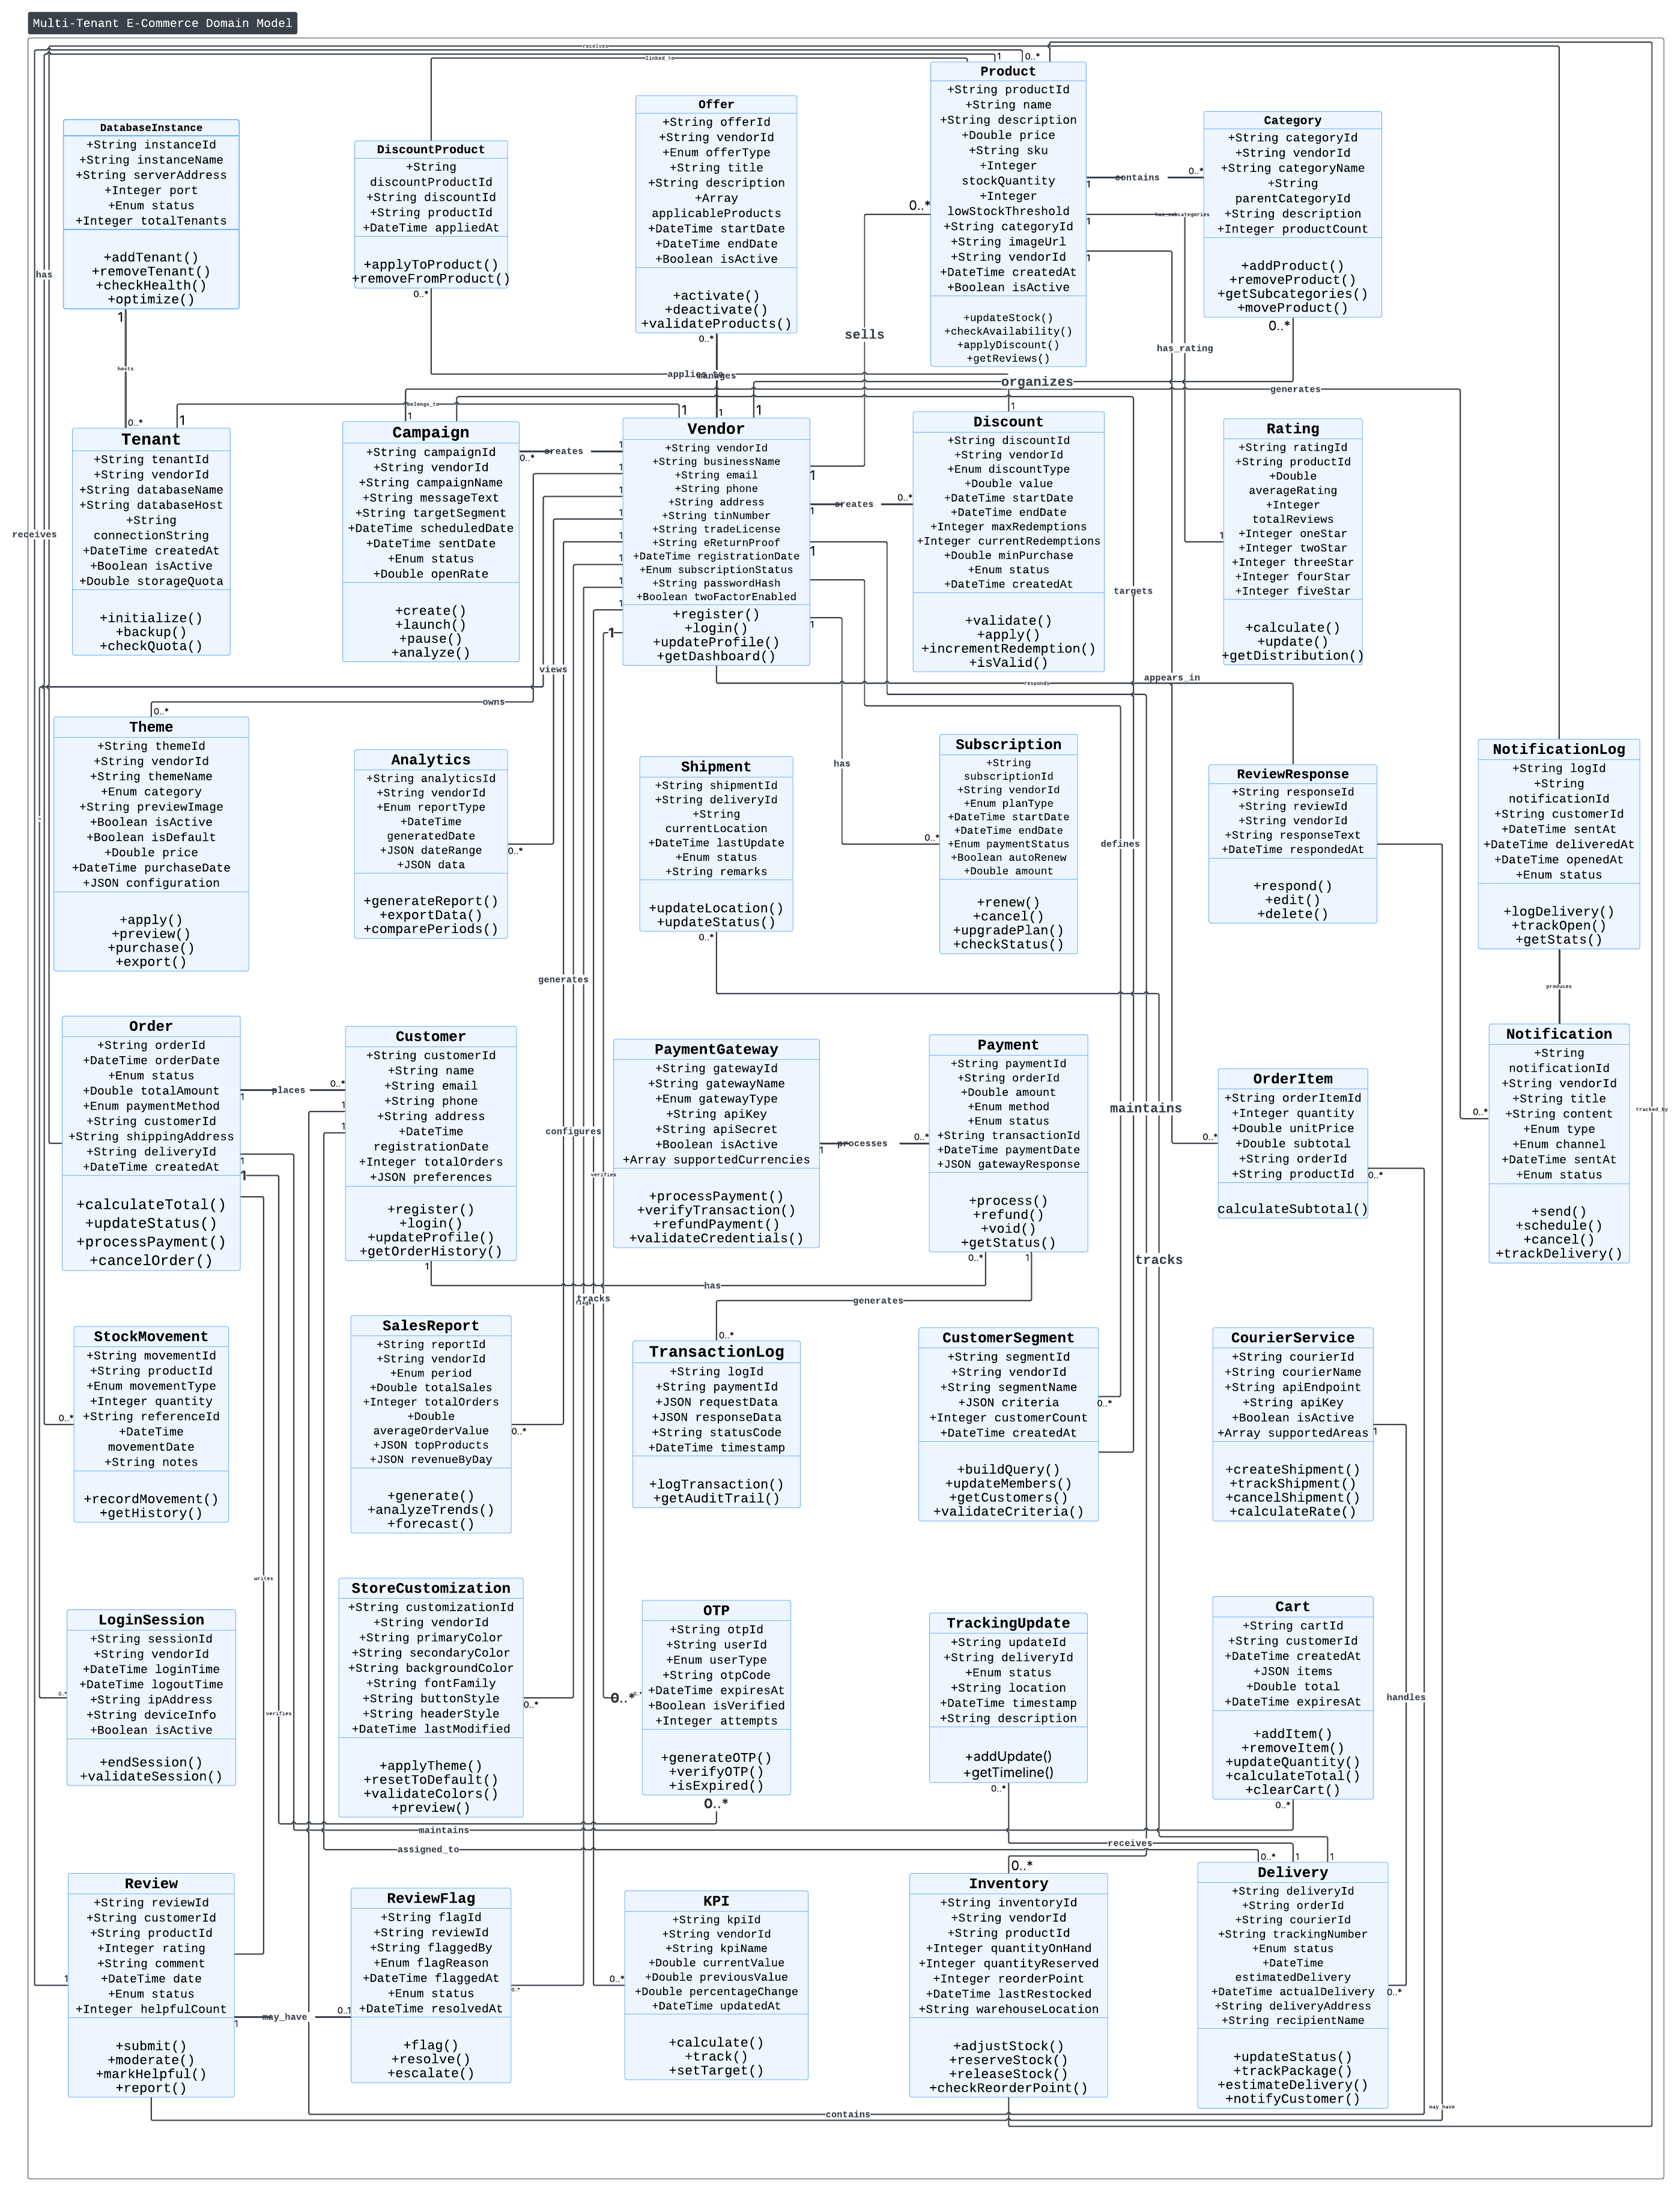
\includegraphics[width=1\linewidth]{figures/ImpLvl UML 5B.png}
    \caption{UML Class Diagram of Multi-tenant E-commerce System (Implementation Level)}
    \label{fig:placeholder}
\end{figure}